\documentclass[12pt, t]{beamer}

\usepackage{graphicx}
\usepackage{amsmath}
\usepackage{setspace}
\usepackage{float} 
\usepackage{multido}
\usepackage{multirow}
\usepackage{array}
\usepackage{enumerate}
\usepackage{booktabs}
\usepackage{indentfirst} 
\usepackage[style=mla]{biblatex}
\usepackage{subcaption}
\usepackage{hyperref}
\usepackage{textpos}

\makeatletter
\let\@@magyar@captionfix\relax
\makeatother

\definecolor{Turquoise3}{RGB}{0, 134, 139}
\renewcommand{\emph}[1]{{\color{Turquoise3}\textsl{#1}}}
\newcommand{\C}{\mathbb{C}} \newcommand{\F}{\mathbb{F}} \newcommand{\R}{\mathbb{R}} \newcommand{\Q}{\mathbb{Q}}
\newcommand{\N}{\mathbb{N}}
\newcommand{\myseries}[2]{$#1_1,#1_2,\dots,#1_#2$}
\newcommand{\nullspace}{~\\[15pt]}
\newcommand{\remark}{\textbf{Remark: }}
\newcommand{\scp}[2]{\langle\,#1\,,\,#2\,\rangle} \newcommand{\scpp}{\langle\,\cdot\,,\,\cdot\,\rangle}


\usetheme{Madrid}
\setbeamertemplate{navigation symbols}{}

\addtobeamertemplate{frametitle}{}{
\begin{textblock*}{100mm}(0.85\textwidth,-1cm)

\includegraphics[height=1cm]{logo.png}
\end{textblock*}}

\definecolor{themecolor}{RGB}{25,25,112} 

\usecolortheme[named=themecolor]{structure}

\setbeamertemplate{items}[default]

\hypersetup{
    colorlinks=true,
    linkcolor=themecolor,
    filecolor=themecolor,      
    urlcolor=themecolor,
    citecolor=themecolor,
}

\title{VV285 RC Part I}
\subtitle{\textbf{Elements of Linear Algebra}\\``Linear Algebra!"}
\institute[UM-SJTU JI]{Univerity of Michigan-Shanghai Jiao Tong University Joint Institute}
\author{Yiwen Tu}

\begin{document}

\begin{frame}
    \titlepage
    \begin{center}
        
\includegraphics[height=2cm]{logo2.png}
    \end{center}
\end{frame}

\begin{frame}
    \frametitle{Something you need to pay attention to...}
    Think More and Be Interactive!
    \begin{itemize}
        \item Do think more about the question in ``()''. \\e.g. ``(How to prove?)''
        \item You are welcome to ask questions in a adequate manner.
        \item DO MORE PRACTICE
    \end{itemize}
    

\end{frame}

\begin{frame}
    
    \frametitle{Overview of Linear Algebra}
    \begin{enumerate}
        \item Systems of Linear Equations
        \item Finite-Dimensional Vector Spaces
        \item Inner Product Spaces
        \item Linear Maps
        \item Matrices
        \item Theory of Systems of Linear Equations
        \item Determinants
    \end{enumerate}
\end{frame}
   
\begin{frame}
    \frametitle{Warm up!}
    Prove or give a counterexample: If $v_1,v_2,v_3,v_4$ is a basis of $V$ and $U$ is a subspace of $V$ such that $v_1,v_2\in U$ and $v_3,v_4\notin U$, then $v_1,v_2$ is a basis of $U$.
\end{frame}

\begin{frame}
    \frametitle{Warm up!}
    Suppose $p_{0}, p_{1}, \ldots, p_{m}$ are polynomials in $\mathcal{P}_{m}(\F)$ such that $p_{k}(2)=0$ for each $k.$ Prove that $p_{0}, p_{1}, \ldots, p_{m}$ is not linearly independent in $\mathcal{P}_{m}(\F)$
\end{frame}

\section{Inner Product Spaces}
\begin{frame}
    \frametitle{Overview - Inner Product Spaces}
    \begin{enumerate}
        \item Inner Product Spaces
        \item Induced Norm
        \item Orthogonality \& Orthonormal System
        \item The Projection Theorem
        \item Gram-Schmidt Orthonormalization
    \end{enumerate}

\end{frame}

\subsection{Inner Product Space}
\begin{frame}[allowframebreaks]
    \frametitle{Inner Product Space}
    Let $V$ be a real or complex vector space. Then a map $\langle\,\cdot\,,\,\cdot\,\rangle: V\times V\rightarrow\F$ is called a scalar product or inner product if for all $u,v,w\in V$ and all $\lambda\in\F$
    \begin{enumerate}
        \item \textit{Positive-definite}\\ $\scp{v}{v}\geq0$ and $\scp{v}{v}=0$ if and only if $v=0$,
        \item \textit{Linearity in the 2nd argument}\\ $\scp{u}{v+w}=\scp{u}{v}+\scp{u}{w}$
        \item \textit{Linearity in the 2nd argument}\\ $\scp{u}{\lambda v}=\lambda\scp{u}{v}$
        \item \textit{Conjugate symmetry}\\ $\scp{u}{v}=\overline{\scp{v}{u}}$
    \end{enumerate}
    The pair $(V,\scpp)$ is called an \emph{inner product space}.
    \newpage
    Prove that
    \begin{enumerate}
        \item \[\scp{\lambda u}{v}=\overline{\lambda}\scp{u}{v}.\]
        \item \[\scp{u+v}{w}=\scp{u}{w}+\scp{v}{w}\]
    \end{enumerate}
    This is called the \emph{conjugate linearity} in the 1st argument.
    \nullspace
    What if $\F=\R$?

    \newpage
    Why is inner product space important?
    \nullspace
    \begin{itemize}
        \item allow the rigorous introduction of intuitive geometrical notions such as the length of a vector or the angle between two vectors
        \item provide the means of defining orthogonality between vectors (zero inner product)
        \item generalize Euclidean spaces (in which the inner product is the dot product, also known as the scalar product) to vector spaces of any (possibly infinite) dimension, and are studied in functional analysis.
        \item  naturally induces an associated \emph{norm}, thus an inner product space is also a \emph{normed vector space}.
    \end{itemize}
\end{frame}

\subsection{Induced Norm}
\begin{frame}[allowframebreaks]
    \frametitle{Induced Norm}
    Let $(V,\scpp)$ be an inner product space. The map
    \[\|\cdot\|:V\rightarrow\R,\qquad\qquad\|v\|=\sqrt{\scp{v}{v}}\]
    is called the \emph{induced norm} on $V$.
    \nullspace
    (How to prove that an induced norm is actually a norm?)

    \begin{figure}[H]
    \centering
    \includegraphics[width=\textwidth]{2020-05-20-13-53-34.png}
    \end{figure}
    
    \newpage
    \begin{itemize}
        \item In $\C^n$ we can define the inner product
            \begin{equation*}
              \scp{x}{y}:=\sum_{i=1}^{n}\overline{x_i}y_i\qquad\qquad
              \qquad x,y\in\C^n.
            \end{equation*}
            \vspace*{-4mm}
        \item In $C([a,b])$, the space of complex-valued, continuous functions on the interval $[a,b]$, we can define an inner product by
            \[\scp{f}{g}:=\int_{a}^{b}\overline{f(x)}g(x)dx,\qquad\qquad
            f,g\in C([a,b]).\]
      \end{itemize}
    \remark Pay attention to the conjugate in two definitions. We will study further on the last one in VV286 to establish \emph{Fourier Series}!

    \newpage
    By \textit{the Cauchy-Schwarz inequality}, we define the \emph{angle} $\alpha(u,v)\in[0,\pi]$ \emph{between u and v} by
    \begin{equation}
        \cos\alpha(u,v)=\frac{\scp{u}{v}}{\|u\|\|v\|}.
    \end{equation}
    We are particularly interested in the case that $\alpha=\pi/2$. i.e. $\scp{u}{v}=0$. Therefore, we introduce \emph{orthogonality}.
\end{frame}

\begin{frame}
    \frametitle{Exercise}
    Try to prove yourself!
    \begin{itemize}
        \item For real inner product space:
        $$<u,v>=\frac{||u+v||^2-||u-v||^2}{4}$$
        \item For inner product spaces $V_1$, $V_2$,... $V_m$,
        $$<(u_1,...u_m),(v_1,...v_m)>=<u_1,v_1>+...+<u_m,v_m>$$
    \end{itemize}
\end{frame}

\subsection{Orthogonality}
\begin{frame}[allowframebreaks]
    \frametitle{Orthogonality}
    Let $(V,\scpp)$ be an inner product vector space.
    \begin{enumerate}[1.]
        \item Two vectors $u,v\in V$ are called \emph{orthogonal} or \emph{perpendicular} if $\scp{u}{v}=0$. We then write $u\perp v$.
        \item We call
              \begin{equation*}
                  M^{\perp}:=\left\{v\in V:\mathop{\forall}_{m\in M}\scp{m}{v}=0\right\}
              \end{equation*}
              the \emph{orthogonal complement} of a set $M\subset V$.
    \end{enumerate}
    For short, we sometimes write $v\perp M$ instead of $v\in M^{\perp}$ or $v\perp m$ for all $m\in M$.
    \nullspace
    \remark The orthogonal complement $M^{\perp}$ is a subspace of $V$.\\
    (How to prove?)
\end{frame}

\begin{frame}[allowframebreaks]
    \frametitle{Orthonormal Systems \& Bases}
    Let $(V,\scpp)$ be an inner product vector space. A tuple of vectors (\myseries{v}{r})$\in V$ is called a \emph{(finite) orthonormal system} if
    \begin{equation*}
        \scp{v_j}{v_k}=\delta_{jk}:=\left\{\begin{aligned}&1\;\;\;\text{for }j=k,\\&0\;\;\;\text{for}~j\neq k,\end{aligned}\right.,\qquad\qquad j,k=1,\ldots,r,
    \end{equation*}
    i.e., if $\|v_k\|=1$ and $v_j\perp v_k$ for $j\neq k$.
    \nullspace
    Let $(V,\scpp)$ be a finite-dimensional inner product vector space and $\mathcal{B}=(e_1,\ldots,e_n)$ a basis of $V$. If $\mathcal{B}$ is also an orthonormal system, we say that $\mathcal{B}$ is an \emph{orthonormal basis} (ONB).\\
    \newpage
     Let $(V,\scpp)$ be a finite-dimensional inner product vector space and $\mathcal{B}=\{e_1,\ldots,e_n\}$ an orthonormal basis of $V$. Then
    \begin{equation*}
        \|v\|^2=\sum_{i=1}^{n}|\scp{v}{e_i}|^2
    \end{equation*}
    for any $v\in V$.
    \nullspace
    \remark Parseval’s Theorem gives a alternative way to calculate a vector's induced norm.
\end{frame}

\begin{frame}
    \frametitle{Linear Functionals on Inner Product Space}
    \emph{A linear functional} on V is a linear map from V to F. In other words, a linear functional is an element of $\mathbf{L}(V,F)$
    \nullspace
    \emph{Example} $$\phi(p)=\int_{-1}^{1} p(t)cos(t) dt$$ is a linear functional on $P_2(R)$
    \nullspace
    \emph{Riesz Representation Theorem} Suppose V is finite-dimensional and $\phi$ is a linear functional on $V$. Then there is a unique vector $u\in V$ such that:
    $$\phi (v)= \langle v,u \rangle $$
\end{frame}

\begin{frame}
    \frametitle{Linear Functionals on Inner Product Space}
    \emph{Riesz Representation Theorem} Suppose V is finite-dimensional and $\phi$ is a linear functional on $V$. Then there is a unique vector $u\in V$ such that:
    $$\phi (v)= \langle v,u \rangle $$

    \textbf{Proof:} 
    
    First we show there exists a vector $u \in V$ such that $phi (v)=\langle v,u \rangle $ for every $v \in V$. Let $e_1,\cdots,e_n$ be an orthornormal basis of $V$. Then
    \begin{equation*}
        \begin{aligned}
            \phi(v)&=\phi (\langle v, e_1\rangle  e_1+...+\langle v, e_n \rangle e_n)\\
                  &=\langle v, e_1\rangle \phi (e_1)+...+\langle v, e_n \rangle \phi (e_n)\\
                  &= \langle v, \overline{\phi (e_1)}e_1+...\overline{\phi (e_n)}e_n \rangle
        \end{aligned}
    \end{equation*}
    for every $v \in V$, where the first equality comes from 6.30. Thus setting
    \begin{equation}
        u=\overline{\phi (e_1)}e_1+\cdots \overline{\phi (e_n)}e_n 
    \end{equation}
  

    
\end{frame}
\begin{frame}
        \frametitle{Linear Functionals on Inner Product Space}
    we have $\phi (v)=\langle v, u \rangle $ for every $v \in V$, as desired.
    Now we prove that only one vector $u \in V$ has the desired behavior.Suppose $u_1$, $u_2\in V$ are such that
    \[
        \phi (v) =\langle v, u_1 \rangle =\langle v, u_2 \rangle
   \]
    for every $v \in V$. Then
    $$
    0=\langle v,u_1 \rangle -\langle v, u_2 \rangle =\langle v, u_1-u_2\rangle
    $$
    for every $v \in V$. Taking $v=u_1-u_2$ shows that $u_1-u_2 =0$. In other words, $u_1=u_2$, completing the proof of the uniqueness part of the result. 
    
\end{frame}
\begin{frame}
    \frametitle{Exercise*}
    For $u \in V$, Let $\phi u$ denote the linear functional on V defined by:
    \[
    (\phi u)(v)=\langle v,u \rangle    
    \]
    \begin{itemize}
        \item Show that if $\textbf{F =R}$, then $\phi$ is a linear map from $V$ to $V^{'}$.
        \item Show that if $\textbf{F =C}$ and V $\neq\{0\}$. then $\phi$ is not a linear map.
        \item Show that $\phi$ is injective.
        \item Suppose $\textbf{F=R}$ and $V$ is finite-dimensional. Use the first and third parts and a dimension-counting argument to show that $\phi$ is isomorphism from $V$ to $V^{'}$
    \end{itemize}
\end{frame}

\subsection{Projection Theorem}
\begin{frame}[allowframebreaks]
    \frametitle{Projection Theorem}
    Let $(V,\scpp)$ be a (possibly infinite-dimensional) inner product vector space and (\myseries{e}{r}), $r\in\N$, be an orthonormal system in $V$. Denote $U:=\text{span}\{e_1,\ldots,e_r\}.$\\
    Then for every $v\in V$ there exists a unique representation
    \begin{equation*}
        v=u+w\multido{}{3}{\qquad}\text{where}~u\in U~\text{and}~w\in U^{\perp}
    \end{equation*}
    and $u=\sum\limits_{i=1}^{r}\scp{e_i}{v}e_i,\,w:=v-u.$
    The vector
    \begin{equation*}
        \pi_Uv:=\sum_{i=1}^{r}\scp{e_i}{v}e_i
    \end{equation*}
    is called the \emph{orthogonal projection} of $v$ onto $U$.\\
    \newpage
    The projection theorem essentially states that \textbf{$\pi_Uv$ always exists} and is independent of the choice of the orthonormal system (it depends only on the span $U$ of the system).
    \nullspace
    Moreover, it generalize the idea of projection:
    $$
        \pi_{e_i}v\rightarrow\pi_Uv
    $$
    A vector in an inner product space can be decomposed not only on its \emph{orthonormal basis} but also on its \emph{subspaces}.
\end{frame}

\subsection{Exercise}

\begin{frame}
    \frametitle{Exercise}
    \begin{itemize}
        \item Prove that $cos(nx)$ are mutually independent
        \item Prove that $sin(nx)$ are mutually independent
        \item Find a set of orthogonal basis
        \item Express function $y=rect(x+2n)$ with the basis you find
    \end{itemize}
\end{frame}

\begin{frame}
    \frametitle{Gram-Schmidt Orthonormalization}
    Just remember how to do it.
    \begin{align*}
         & w_{1}:=\dfrac{v_{1}}{\left\|v_{1}\right\|}                                                                                                                                                 \\
         & w_{k}:=\dfrac{v_{k}-\sum_{j=1}^{k-1}\left\langle w_{j}, v_{k}\right\rangle w_{j}}{\left\|v_{k}-\sum_{j=1}^{k-1}\left\langle w_{j}, v_{k}\right\rangle w_{j}\right\|}, \quad k=2, \ldots, n
    \end{align*}
    \nullspace
    How to use Gram-Schmidt Orthonormalization to obtain \textit{Legendre polynomials}?
\end{frame}

\subsection{Linear Maps}
\begin{frame}
    \frametitle{Linear Map}
    A map $L: U \leftarrow V$ is said to be \emph{linear} if it is both 
    
    \emph{homogeneous}, i.e. 
    \[
    L(\lambda u)=\lambda L(u)    
    \]
    
    \emph{additive},i,e.
    \[
    L(u+v)=L(u)+L(v)    
    \]
    
    \emph{structural-perserving}
    \nullspace
    \begin{center}
    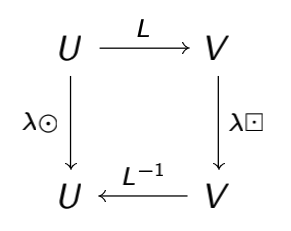
\includegraphics[width=0.2\textwidth]{sp.png}
    \end{center}
\end{frame}

\begin{frame}
    \frametitle{Linear Map}
    \emph{Examples}
    \begin{itemize}
        \item  We let 0 denote the function that takes each element of some vector space to the additive identity of another vector space.
        \[
        0v=0    
        \]
        \item The $\emph{identity map}$, denoted $I$, is the function on some vector space that takes each element to itself. 
         \[
         Iv=v
         \]
         \item Define $D \in L(P(R),P(R)) $ by
         \[
         Dp=p^{'}    
         \]
    
         \item $\emph{backward shift}$
         
         Define $T \in L(F^{\infty},F^{\infty}) $ by
         \[
         T(x_1,x_2,x_3,\cdots)=(x_2,x_3,x_4,...)    
         \]
    \end{itemize}
\end{frame}

\begin{frame}
    \frametitle{Linear Map}
    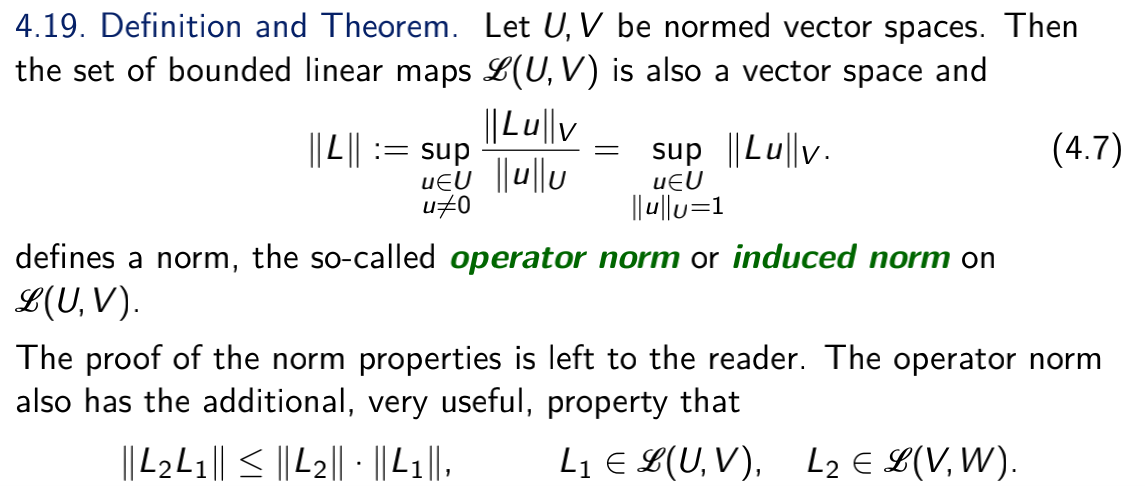
\includegraphics[width=\textwidth]{1}
    \nullspace
    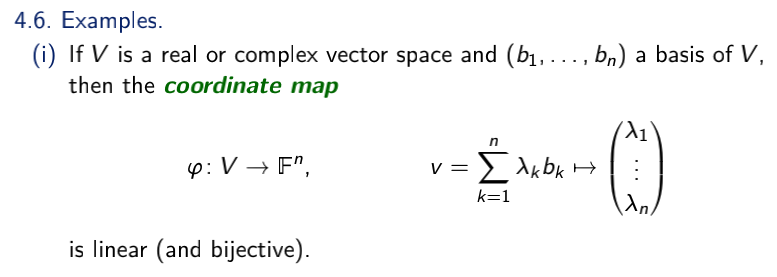
\includegraphics[width=\textwidth]{2}
\end{frame}

\begin{frame}
    \frametitle{Linear Map}
    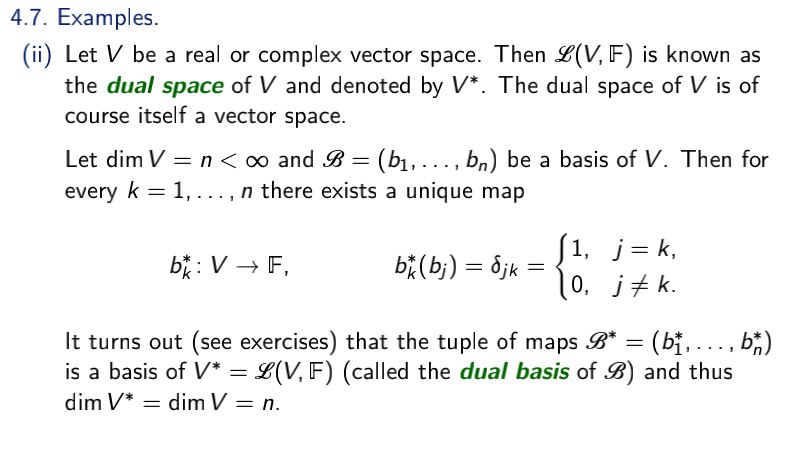
\includegraphics[width=\textwidth]{3}
\end{frame}

\begin{frame}
    \frametitle{Linear Map}
    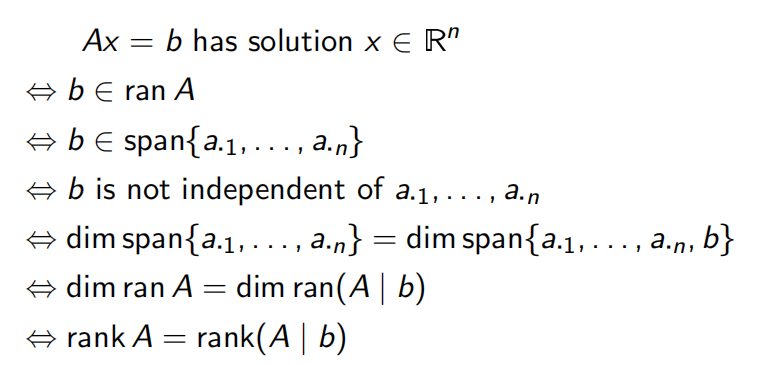
\includegraphics[width=\textwidth]{4}
    \nullspace
    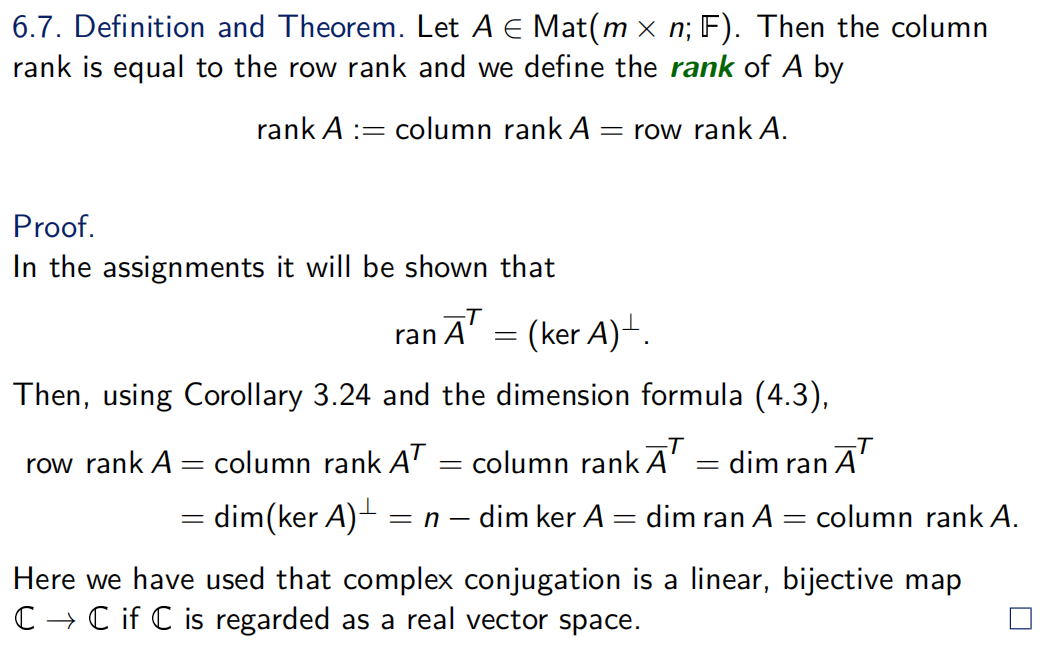
\includegraphics[width=\textwidth]{5}
\end{frame}

\begin{frame}
    \frametitle{Linear Map}
    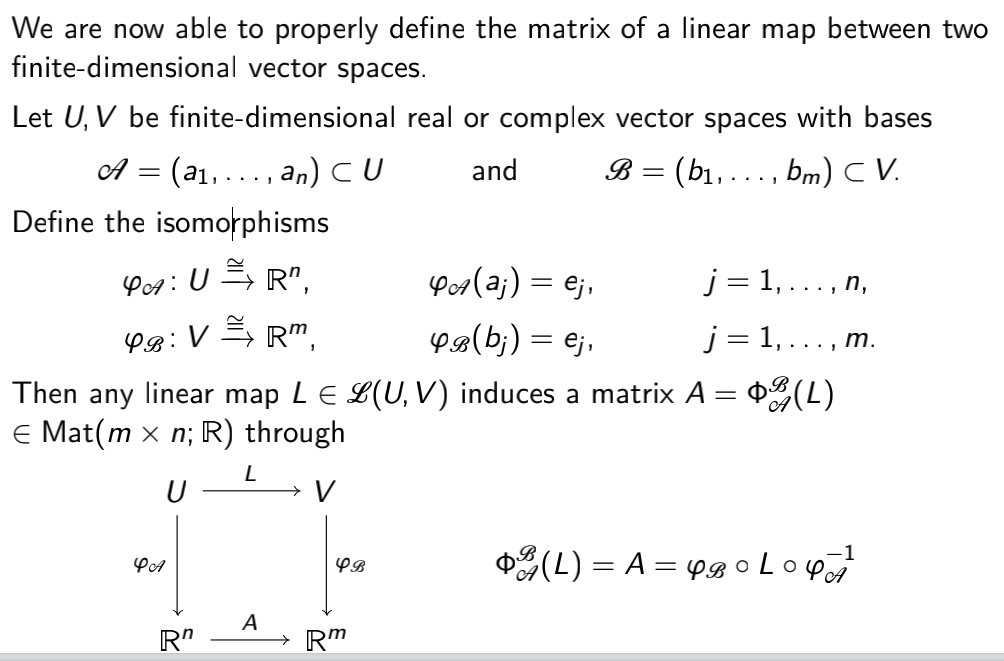
\includegraphics[width=\textwidth]{6}
    \nullspace
    
\includegraphics[width=\textwidth]{7}
\end{frame}
\begin{frame}
    \frametitle{Linear Map}
    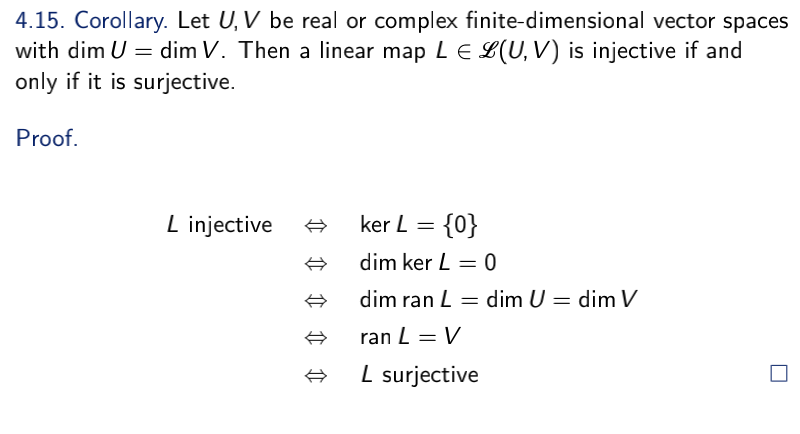
\includegraphics[width=\textwidth]{8}
\end{frame}

\begin{frame}
    \frametitle{Linear Map}
    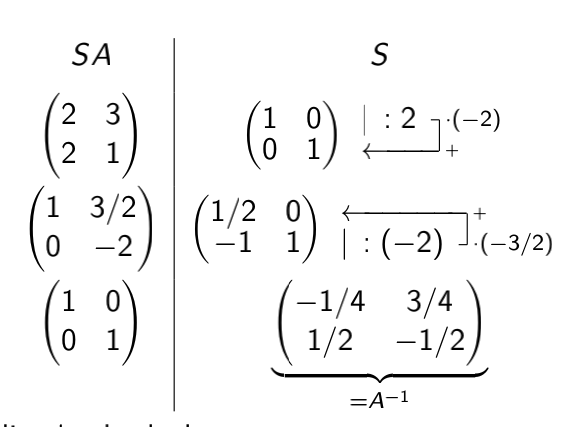
\includegraphics[width=\textwidth]{9}
\end{frame}
\begin{frame}
    \frametitle{Exercise}
    Give an example of a function $\phi: C\rightarrow C$ such that
    \[
    \phi (w+z)=\phi(w)+\phi(z)    
    \]
    for all $w,z \in C$ but $\phi$ is not linear. Here C is a complex vector space.
\end{frame}

\begin{frame}
    \frametitle{Exercise}


Suppose $v_2,...,v_m$ is a linearly dependent list of vectors in $V$. Suppose also that $W\neq$ \{0\}. Prove that there exist $w_1,\cdots,w_m \in W$ such that no $T\in L(V,W)$ satisfies $Tv_k =w_k$ for each k=1,...m.
\end{frame}
\begin{frame}
\frametitle{Injectivity and Surjectivity}
A function $T: V \rightarrow W$ is called \emph{injective} if Tu=Tv imples u=v

A function $T: V \rightarrow W$ is called \emph{injective} if ker$T$=\{0\}

A function $T: V \rightarrow W$ is called \emph{surjective} if ran$T\textrm{=}W$

Suppose V and W are finite-dimensional vector spaces such that dimV $\textgreater$ dimW. Then no linear map from V to W is injective.
   
Suppose V and W are finite-dimensional vector spaces such that dimV $\textless$ dimW. Then no linear map from W to V is surjective.
\end{frame}
\begin{frame}
    \frametitle{Discussion}
    \vspace{1.5cm}
    \Large
    \centering
    Learn Well\\
    And\\
    Have Fun!\\


\end{frame}

\end{document}